\documentclass[12pt,]{article}
\usepackage{lmodern}
\usepackage{amssymb,amsmath}
\usepackage{ifxetex,ifluatex}
\usepackage{fixltx2e} % provides \textsubscript
\ifnum 0\ifxetex 1\fi\ifluatex 1\fi=0 % if pdftex
  \usepackage[T1]{fontenc}
  \usepackage[utf8]{inputenc}
\else % if luatex or xelatex
  \ifxetex
    \usepackage{mathspec}
  \else
    \usepackage{fontspec}
  \fi
  \defaultfontfeatures{Ligatures=TeX,Scale=MatchLowercase}
\fi
% use upquote if available, for straight quotes in verbatim environments
\IfFileExists{upquote.sty}{\usepackage{upquote}}{}
% use microtype if available
\IfFileExists{microtype.sty}{%
\usepackage{microtype}
\UseMicrotypeSet[protrusion]{basicmath} % disable protrusion for tt fonts
}{}
\usepackage[margin=1.0in]{geometry}
\usepackage{hyperref}
\hypersetup{unicode=true,
            pdfborder={0 0 0},
            breaklinks=true}
\urlstyle{same}  % don't use monospace font for urls
\usepackage{graphicx,grffile}
\makeatletter
\def\maxwidth{\ifdim\Gin@nat@width>\linewidth\linewidth\else\Gin@nat@width\fi}
\def\maxheight{\ifdim\Gin@nat@height>\textheight\textheight\else\Gin@nat@height\fi}
\makeatother
% Scale images if necessary, so that they will not overflow the page
% margins by default, and it is still possible to overwrite the defaults
% using explicit options in \includegraphics[width, height, ...]{}
\setkeys{Gin}{width=\maxwidth,height=\maxheight,keepaspectratio}
\IfFileExists{parskip.sty}{%
\usepackage{parskip}
}{% else
\setlength{\parindent}{0pt}
\setlength{\parskip}{6pt plus 2pt minus 1pt}
}
\setlength{\emergencystretch}{3em}  % prevent overfull lines
\providecommand{\tightlist}{%
  \setlength{\itemsep}{0pt}\setlength{\parskip}{0pt}}
\setcounter{secnumdepth}{5}
% Redefines (sub)paragraphs to behave more like sections
\ifx\paragraph\undefined\else
\let\oldparagraph\paragraph
\renewcommand{\paragraph}[1]{\oldparagraph{#1}\mbox{}}
\fi
\ifx\subparagraph\undefined\else
\let\oldsubparagraph\subparagraph
\renewcommand{\subparagraph}[1]{\oldsubparagraph{#1}\mbox{}}
\fi

%%% Use protect on footnotes to avoid problems with footnotes in titles
\let\rmarkdownfootnote\footnote%
\def\footnote{\protect\rmarkdownfootnote}

%%% Change title format to be more compact
\usepackage{titling}

% Create subtitle command for use in maketitle
\providecommand{\subtitle}[1]{
  \posttitle{
    \begin{center}\large#1\end{center}
    }
}

\setlength{\droptitle}{-2em}

  \title{\vspace{2in} \textbf{\underline{An Application of Self Organizing Maps}}}
    \pretitle{\vspace{\droptitle}\centering\huge}
  \posttitle{\par}
  \subtitle{\vspace{0.35in} \textbf{Methods Paper}\\
\vspace{0.25in} Lee Panter\\
\vspace{0.05in} The University of Colorado-Denver\\
\vspace{0.05in} Department of Mathematical and Statistical Sciences\\
\vspace{0.05in} Math 6330: Workshop in Statistical Consulting}
  \author{}
    \preauthor{}\postauthor{}
    \date{}
    \predate{}\postdate{}
  
\usepackage{amsmath}
\usepackage{amsfonts}
\usepackage{amssymb}
\usepackage{enumitem}
\usepackage{graphicx}
\usepackage{array}
\usepackage{epsfig}
\usepackage{color}
\usepackage{multirow}
\usepackage{amsrefs}
\usepackage{placeins}
\usepackage[utf8]{inputenc}
\usepackage[english]{babel}
\usepackage{multicol}
\usepackage{comment}
\usepackage{multirow}
\usepackage{indentfirst}
\usepackage{listings}
\usepackage{setspace}
\usepackage{wrapfig}
\usepackage[right]{lineno}

\doublespacing
\setlength\parindent{15pt}
\setlength{\parskip}{3mm plus 1mm minus 1mm}

\lstset{frame=tb,
language=R,
aboveskip=3mm,
belowskip=3mm,
showstringspaces=false,
columns=flexible,
numbers=none,
keywordstyle=\color{blue},
numberstyle=\tiny\color{gray},
commentstyle=\color{dkgreen},
stringstyle=\color{mauve},
breaklines=true,
breakatwhitespace=true,
tabsize=3
}

\begin{document}
\maketitle

\thispagestyle{empty}

\newpage

\thispagestyle{empty}

\setcounter{secnumdepth}{4}
\setcounter{tocdepth}{4}
\begin{singlespace}
\tableofcontents
\end{singlespace}

\newpage

\pagenumbering{arabic}

\hypertarget{introduction}{%
\section{Introduction}\label{introduction}}

Self Organizing Maps (SOMs) are hybrid statistical learning algorithms
first introduced by Dr.~Kohonen Teuvo in 1982 in his paper
``Self-organized formation of topologically correct feature maps''
{[}1{]}. SOMs are best characterized as hybrid processes because they
are useful for unsupervised learning in the absence of outcome
information; and once this information has been made available, SOMs can
be extended into classification algorithms. SOMs are used extensively
for clustering, classification, pattern recognition, segmentation and
visualization {[}2{]}.

\hypertarget{background}{%
\subsection{Background}\label{background}}

Self Organizing Maps emulate biological information processing in the
human brain, specifically with respect to compartmentalized processing.
The human brain has dedicated neuronal pathways designed to process
specific stimuli. Signals and inputs will be processed in completely
separate areas of the brain based upon whether they have sensory,
memory, or regulatory effects. The human brain pre-processes inputs,
organizing them into similar clusters prior to evaluation.

Statistical learning algorithms are established as solid platforms for
regression, prediction, and classification. Familiar approaches use
bi-directional information flow, which consequently resembles ``learning
by example''. Algorithms are provided ``examples'' (data) and the
algorithms are corrected until reasonable answers are provided. Although
useful, these bi-directional flow algorithms have shown a tendency to be
input-sensitive; and in theory, this type of learning is not replicating
human intelligence. {[}3{]}

A closer approximation to human intelligence would be an algorithm that
learned by observation. Learning by observation would require an
algorithm to improve outcomes without back propagation of information
from a response {[}3{]}. SOMs are feed-forward algorithms, that improves
outcomes using a three-step approach: Competition, Cooperation, and
Adaptation.

\hypertarget{objective-and-outcome}{%
\subsection{Objective and Outcome}\label{objective-and-outcome}}

The SOM algorithm is useful as an unsupervised method for clustering,
and generating visualizations of high-dimensional data that can be used
for inference since the dimension-reduction methods preserve the
topological characteristics of the high dimensional relationships in the
lower-dimensional representations.

In clustering applications Self Organizing Maps are useful for
developing an understanding how the whole data set, represented as a
large, highly variable population can be represented as a set of
smaller, more homogeneous sub-populations. Visualizations can also show
how the high dimensional representations of the data compare across each
group.

The SOM algorithm is also useful for classifying high dimensional inputs
into low-dimensional outcomes. The process of constructing clusters and
high dimensional visualizations has ``trained'' a SOM map so that new,
unseen observations are readily associated to the same outcome space.

The low-dimensional groupings that are the result of the SOM are further
useful as the input layer of an Artificial Neural Network {[}4{]}. This
approach is a useful data reduction and efficiency measure employed in
training extensive deep learning algorithms. As an alternative
representation of the original observations, a variety of techniques can
be applied to these values.

Self Organizing Maps are useful for characterizing observational
tendencies, and predictor relationships even when no outcome is present
and/or when non-linear techniques are needed. The SOM algorithm can
assist in visualizing relationships in high dimensional spaces, and is
used as a data reduction method for inputs to Artificial Neural
Networks.

SOMs are useful when an order structure can be associate with the
predictor space. This situation is common in cases where predictor
variables are measurements of the same ``type'' of variable. Some
examples of these predictor spaces would include:

\begin{itemize}
\tightlist
\item
  10 questions with integer-valued answers
\item
  Measurements of height, width, and length
\item
  Sports statistics with player percentage values
\end{itemize}

The SOM algorithm heuristically calls for 10\% of the total observation
count as a starting point for the number of lower-dimensional clusters
used. This implies that SOMs require a minimum of around 20 total
observations (two nodes for classification). It should be noted that
Self Organizing Maps are dependent on initialization parameters. Results
can be dependent on parameters provided to the algorithm and convergence
issues.

\hypertarget{case-study-description}{%
\section{Case Study Description}\label{case-study-description}}

\hypertarget{data}{%
\subsection{Data}\label{data}}

An application of a Self Organizing Map will be applied to Edgar
Anderson's Iris Data. This data contains 150 observations of three
species of Iris flowers. The three species of flowers are Iris Setosa
(denoted ``S''), Versicolor (denoted ``Ve''), and Virginica (denoted
``Vi''). There are 50 instances of each species type. There are four
quantitative measurements in addition to species, corresponding to
lengths on the flowers. A summary table of the measurements separated by
species is listed in Table 1 below.

\begin{table}[!h]
\centering
\begin{tabular}{|c|c|cccc|}
\hline
Species                 & Measurement       & Min   & Median & Mean   & Max    \\
\hline
S                       & Sepal Length      & 4.3   & 5      & 5.006  & 5.8    \\ 
S                       & Sepal Width       & 2.3   & 3.4    & 3.428  & 4.4    \\ 
S                       & Pedal Length      & 1     & 1.5    & 1.462  & 1.9    \\ 
S                       & Pedal Width       & 0.1   & 0.2    & 0.246  & 0.6    \\ 
S                       & Sum of Values     & 8.4   & 10.2   & 10.14  & 12     \\ 
S                       & Product of Values & 1.419 & 5.151  & 6.457  & 16.8   \\ 
\hline
Species                 & Measurement       & Min   & Median & Mean   & Max    \\
\hline
Ve                      & Sepal Length      & 4.9   & 5.9    & 5.936  & 7      \\
Ve                      & Sepal Width       & 2     & 2.8    & 2.77   & 3.4    \\
Ve                      & Pedal Length      & 3     & 4.35   & 4.26   & 5.1    \\
Ve                      & Pedal Width       & 1     & 1.3    & 1.326  & 1.8    \\
Ve                      & Sum of Values     & 11.5  & 14.35  & 14.29  & 16.4   \\
Ve                      & Product of Values & 35    & 92.72  & 97.35  & 170.85 \\
\hline
Species                 & Measurement       & Min   & Median & Mean   & Max    \\
\hline
Vi                      & Sepal Length      & 4.9   & 6.5    & 6.588  & 7.9    \\
Vi                      & Sepal Width       & 2.2   & 3      & 2.974  & 3.8    \\
Vi                      & Pedal Length      & 4.5   & 5.55   & 5.552  & 6.9    \\
Vi                      & Pedal Width       & 1.4   & 2      & 2.026  & 2.5    \\
Vi                      & Sum of Values     & 13.6  & 17.2   & 17.14  & 20.4   \\
Vi                      & Product of Values & 93.71 & 228.2  & 227.45 & 431.29 \\
\hline
\end{tabular}
\caption[Iris Data Summary Table]{Summary of Iris case Study Data.}
\end{table}

\textit{Sum of Values} and \textit{Product of Values} are calculated by
performing the corresponding operation (sum or product) on all four
measurements (Sepal Length, Sepal Width, Pedal Length, and Pedal Width)
within each observation. The values of \textit{Sum of Values} and
\textit{Product of Values} are plotted against all four measurements and
against each other in Appendix A.

The data be downloaded directly from the CRAN website by loading the
\texttt{datasets} package and loading \texttt{data(iris)} into the R
working environment.

\hypertarget{case-study-objectives}{%
\subsection{Case Study Objectives}\label{case-study-objectives}}

In an effort to outline the process and potential benefits of using Self
Organizing Maps, a \(4 \times 4\) SOM will be trained on a subset of the
Iris data. This SOM will be used to obtain visualizations of the 16
clusters. Following this clustering, a hierarchy will be imposed on the
16 clusters, and as set of three clusters formed from the hierarchy will
be ordered, and chosen to represent the three Species in the Iris data.
The remaining observations (leftover from the original data after
training) will then be mapped to these ``Synthetic Species'' and an
accuracy estimate will be obtained.

\begin{center}\rule{0.5\linewidth}{\linethickness}\end{center}

\hypertarget{model-and-methods}{%
\section{Model and Methods}\label{model-and-methods}}

\hypertarget{topology-preserving-maps}{%
\subsection{Topology Preserving Maps}\label{topology-preserving-maps}}

Suppose that \((X, d_{X})\) and \((Y, d_{Y})\) are Metric Spaces and
that the observation,
\newline \(\mathbf{x}_{i} = \left( x_{i1}, \ldots, x_{iP} \right)\)
resides in the predictor space, where \(i = 1, \ldots, N\) represents
the number of observations.

A Self Organizing Map is a function that preserves the relationships
between elements in a topological space {[}5{]}.
\[\mathbf{F}: (X, d_{X}) \subseteq \mathbb{R}^{P} \longrightarrow  (Y, d_{y}) \subseteq \mathbb{R}^{Q}\]
where \(Q=1,2\), is the outcome space used for visualization.

Since continuous functions preserve topological relationships, it is
sufficient to require:
\[\forall \epsilon>0, \ \exists \delta>0: \ \mathbf{F}\left(B_{\delta}\left(a\right) \right) \subset B_{\epsilon}\left(\mathbf{F}(a)\right)  \]
where
\[B_{\delta}\left(a\right)  = \left \{ x \in (X, d_{x}) : d_{x}\left(a,x \right) < \delta  \right \}\]
and
\[B_{\epsilon}\left(\mathbf{F}(a\right))  = \left \{ y \in (Y, d_{y}) : d_{y}\left(\mathbf{F}(a),\ y \right) < \epsilon  \right \}\]

\hypertarget{algorithm}{%
\subsection{Algorithm}\label{algorithm}}

Let the outcome space, \(\left(Y, d_{Y} \right)\) be an \((M \times K)\)
lattice structure with nodes enumerated sequentially, so that node
\(j \in \left \{ 1, \ldots, M \times K \right \}\)

\clearpage

\begin{figure}[!h]
\begin{center}
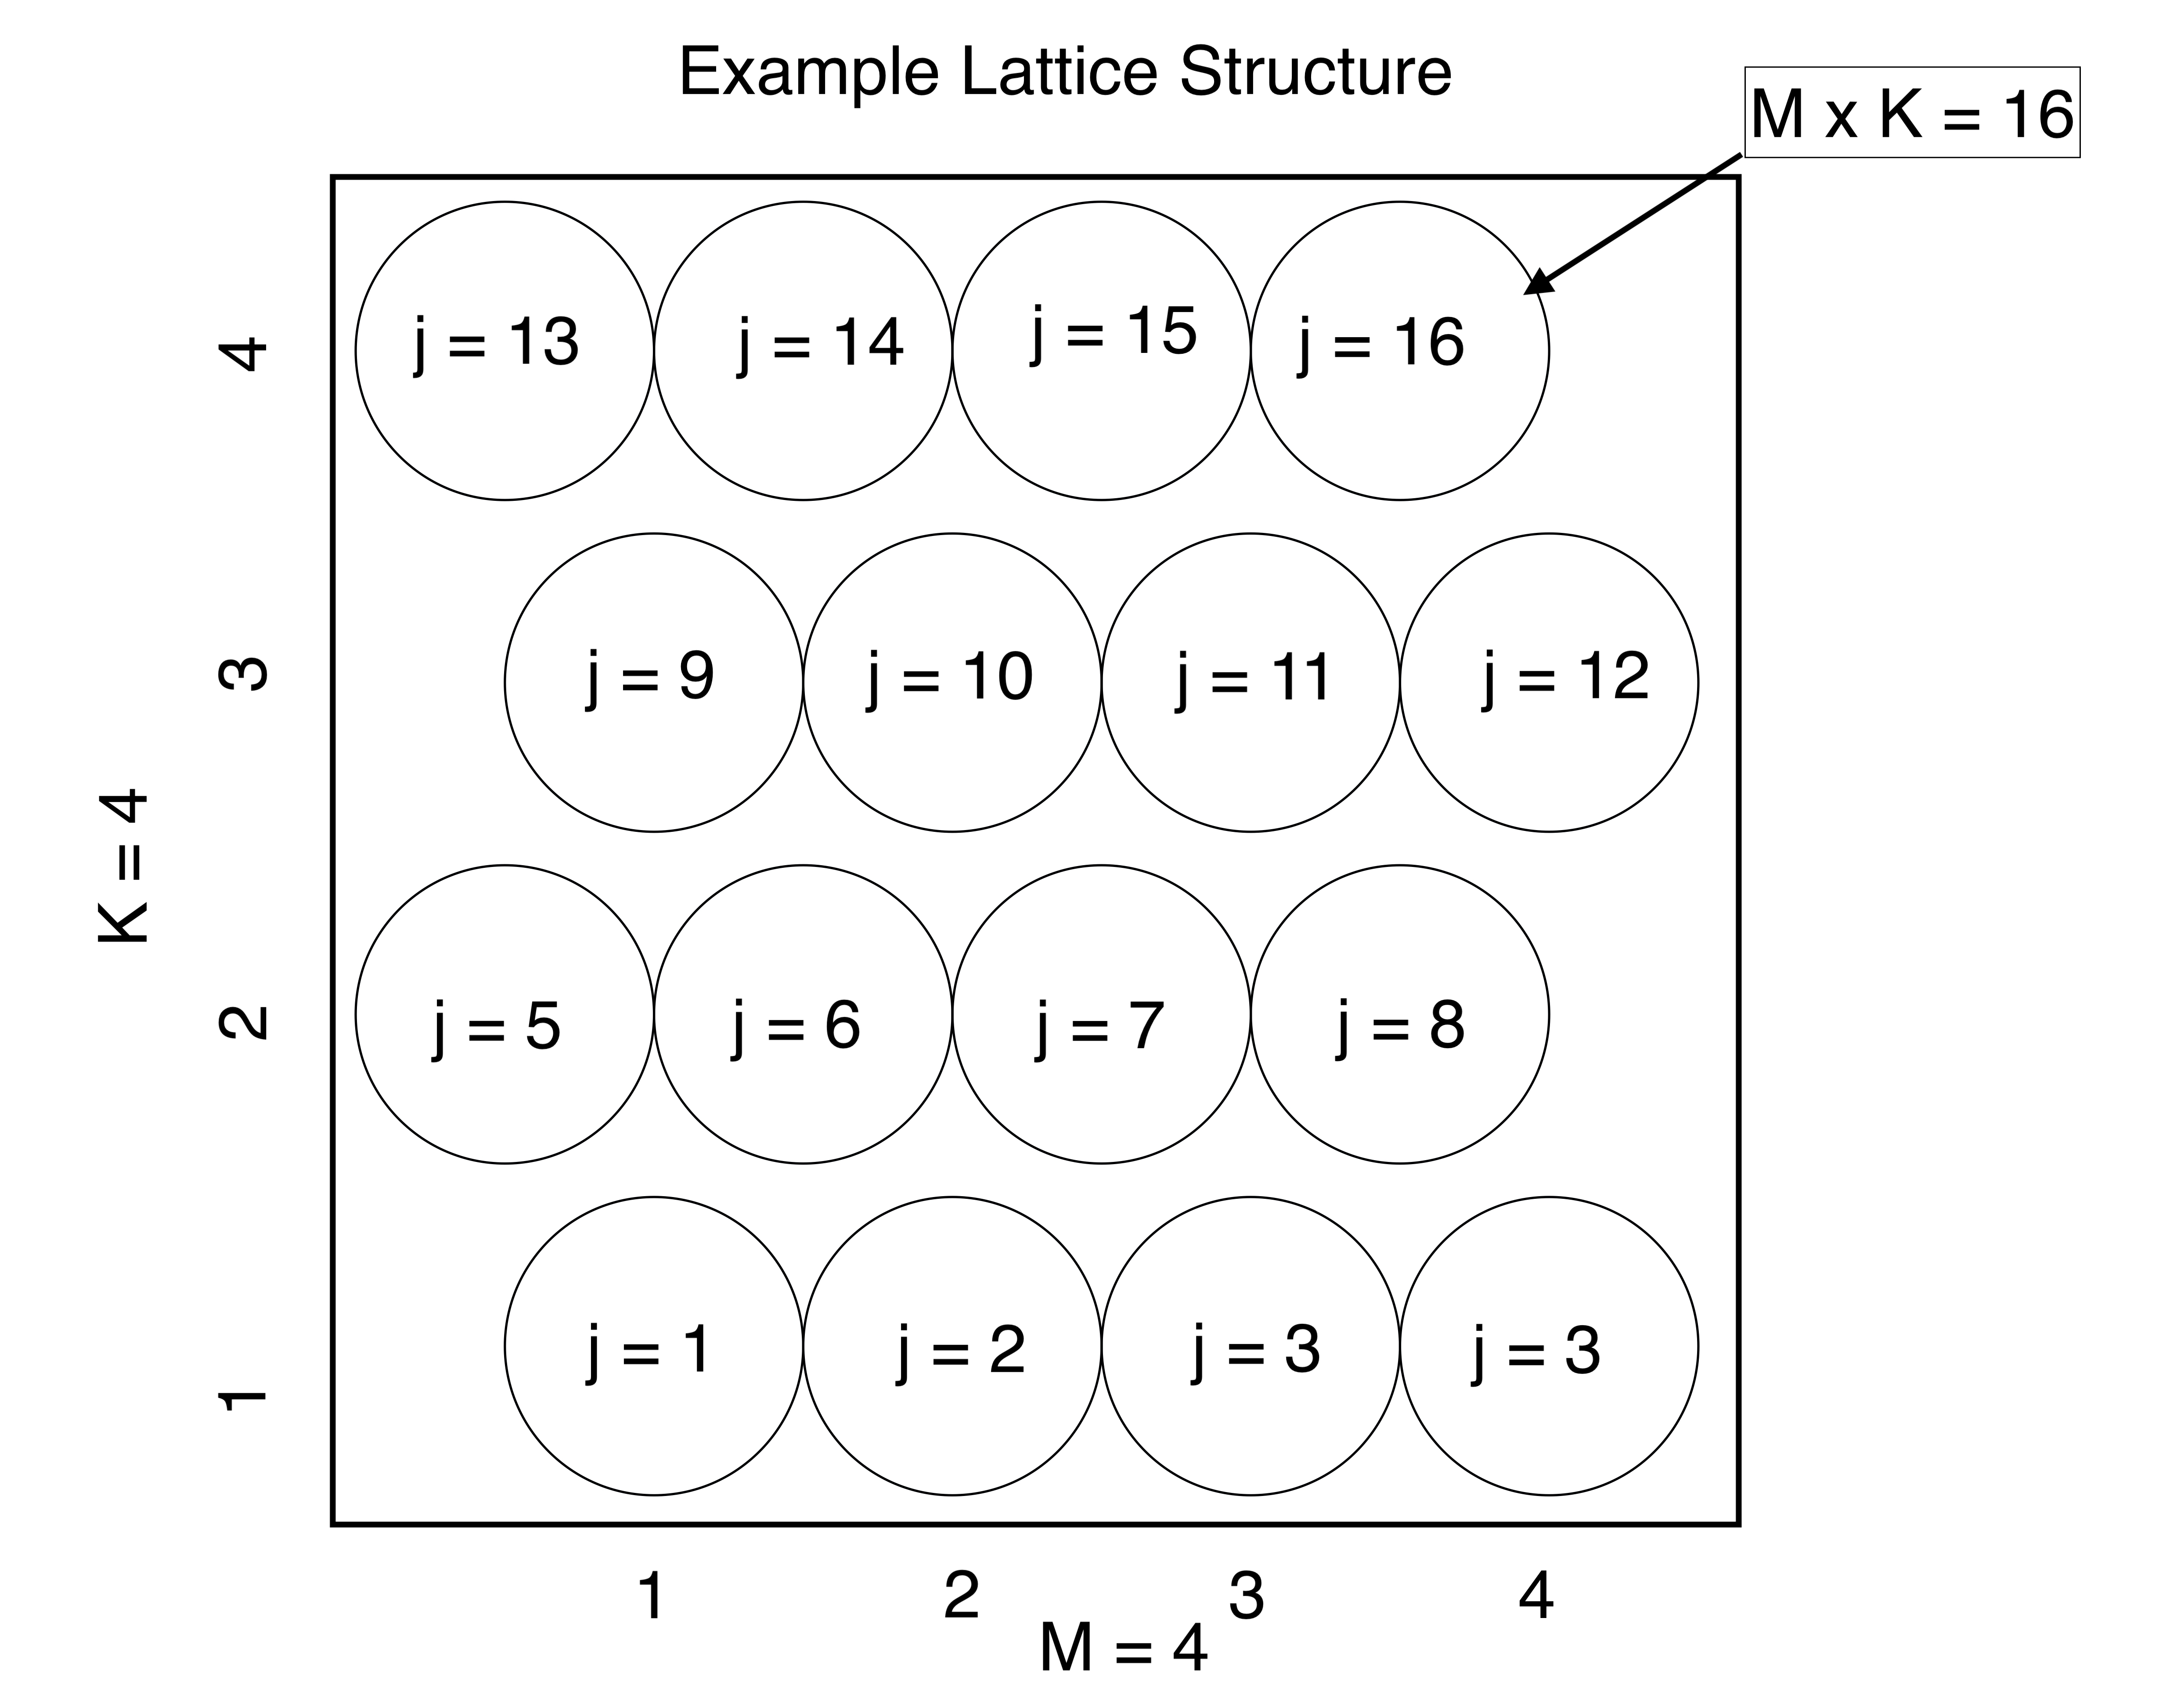
\includegraphics[width=0.5\textwidth]{LatticeEnumeration.jpg}
\end{center}
\caption[Lattice Enumeration Method]{Counting two dimensional lattice structures $j \in \left \{ 1, \ldots, M \times K     \right \}$}
\end{figure}

For each node there will be a weight vector, \(\mathbf{W}_{ij}\)
associated with each outcome:
\[\mathbf{W}_{ij}=\left(W_{ij1}, \ldots, W_{ijP} \right) \] for
\(i = 1, \ldots, N\) and \(j = 1, \ldots, M \times K\), a total of
\(N \times M \times K\) weight vectors.

The weight vectors are adjusted in a three step process, and the process
is repeated until sufficient weights do not move, or move very little
with additional iteration.

In each iteration, a single observation is fed into the algorithm, then
output lattice structure (nodes) and the weights associated with them:

\begin{enumerate}
\def\labelenumi{\arabic{enumi}.}
\tightlist
\item
  \textbf{Compete} for selection as the ``winner'' that maximizes
  proximity within the \textit{output lattice}, which then
\item
  \textbf{Cooperates} with the other output nodes to varying degrees
  according to a neighborhood function. Nodes closer to the winning node
  are adjusted more than those considered further away from it.
\item
  \textbf{Adapt} the weights of the output nodes, adjusting the values
  so that they become more similar to the winning value.
\end{enumerate}

\hypertarget{competition}{%
\subsubsection{Competition}\label{competition}}

Given a single observation
\(\mathbf{x}_{i} = \left( x_{i1}, \ldots, x_{iP} \right)\) where
\(i\in\left \{ 1, \ldots, N\right \}\) weight values are calculated for
each value of \(j = 1, \ldots, M \times K\)
\[\mathbf{W}_{ij}= d_{X} \left( \mathbf{x}_{i}, \mathbf{W}_{j} \right)\]
and a value of \(\mathbf{W}_{i}^*\) is defined based upon:
\[\mathbf{W}_{i}^*=\underset{j}{\arg\min} \ \ d_{X} \left( \mathbf{x}_{i}, \mathbf{W}_{j} \right) \]
this is called the ``winning node''

\hypertarget{cooperation}{%
\subsubsection{Cooperation}\label{cooperation}}

A neighborhood function \(h_{i^{*}}(j, \epsilon(t), \alpha(t))\) to
determine how many (and which) node weights in the vicinity of \(i^{*}\)
will be altered, where \(t=0,1,2\) represents the algorithm iteration
number (discrete time).

\(N_{\epsilon(t_{0})}(i^{*})\) is an open epsilon-ball around \(i^{*}\)
at time \(t=t_{0}\) is the set of nodes given by:

\[N_{\epsilon(t_{0})}(i^{*})=\left \{ j \in 1, \ldots, M \times K \ | \  d_{Y}(i^{*}, j)<\epsilon(t) \right \}\]
\(\epsilon(t)\) is a monotonically decreasing function of \(t\) that
represents the largest cross-sectional width/radius of
\(N_{\epsilon}(i^{*})\).

\(\alpha(t)\) is a monotonically decreasing function of \(t\) that
represents the learning rate.
\(\alpha(t) \in [0,1] \ \forall t\in \mathbb{N}\)

Two neighborhood functions are: \[
h_{i^{*}}(j, \epsilon(t), \alpha(t))=
\begin{cases}
  h_{i^{*}}(j, \epsilon(t), \alpha(t)) & \text{if}  \quad j \in N_{\epsilon}(i^{*}) \\ 
  0 & \text{if} \quad   j  \notin N_{\epsilon}(i^{*}) 
\end{cases}
\]

or they can be continuous, as in:
\[h_{i^{*}}(j, \epsilon(t), \alpha(t)) = exp \left( \frac{-d^{2}(i^{*}, j)}{2\epsilon^{2}(t)} \right) \]
\(\forall j \in \left \{ 1, \ldots,M \times K\right \}\)

\hypertarget{adaptation}{%
\subsubsection{Adaptation}\label{adaptation}}

Following the calculations of the winner \(\mathbf{W}_{i}^{*}\) and
weights \(\mathbf{W}_{ij}\), the neighborhood calculations
\(h_{i^{*}}(j, \epsilon(t), \alpha(t))\) the set of weights are updated
to reflect the information gained by minimizing the distance (the
competition step), using the update formula:
\[\mathbf{W}_{ij}^{t_{1}} = \mathbf{w}_{ij}^{t_{0}} + \alpha(t_{0}) \times  h_{i^{*}}(j, \epsilon(t_{0}), \alpha(t_{0})) \left [ \mathbf{x}(t_{0})-\mathbf{W}_{ij}^{t_{0}}    \right ]\]
for each value of \(j=1, \ldots, M \times K\)

where the discrete time step is defined as \(t_{1} = t_{0} + 1\), and
the algorithm is repeated over the discrete time variable until
convergence is seen in the weights for each value observation, and the
Competition, Cooperation, and Adaptation portions of the algorithm are
repeated for each observation in the data until convergence is seen in
the output layer. Re-circulations through the data set may also be
needed.

\hypertarget{assumptions}{%
\subsection{Assumptions}\label{assumptions}}

One of the major benefits of implementing Self Organizing Maps is a
general lack of assumptions. The SOM algorithm is dependent on being
able to order observations within the predictor space, which means that
there can only be limited unordered categorical values. Response values
that cannot be associated with a magnitude or generalized hierarchy are
not well suited to comparison, and alternative methods must be
considered. Additionally, the SOM algorithm makes an implicit assumption
that inputs are equally weighted prior to training. This assumption is
critical to the related assumption that weight values are bounded, and
restricts the types of data that the SOM algorithm can accommodate
further to data that is standardizable.

Predictors and additional covariate information should be considered in
close coordination with the definition of metrics chosen for the
underlying mapping input and output spaces. Data with order can be
accommodated, even if the the values are not quantitative, but careful
metric definitions be evaluated.

The SOM algorithm is extremely flexible with respect to parametric
assumptions. SOMs do not assume any properties of a distribution prior
to mapping or clustering observations. This lack of a distributional
assumption makes SOMs a particularly useful tool for data with missing
observations. SOMs construct mappings based on empirical distributions
that contain all informational attributes in the data (even those that
are missing). In this way, a missing value is considered information
itself.

\begin{center}\rule{0.5\linewidth}{\linethickness}\end{center}

\newpage

\hypertarget{analysis-and-results}{%
\section{Analysis and Results}\label{analysis-and-results}}

A \(4X4\) Self Organizing Map is fit to normalized Iris data, using a
hexagonal topology arrangement of the output node layer. The SOM fitting
process was restricted to 400 epochs (iterations through the entire data
set). The SOM mapping is displayed below in Figure 2:

\begin{figure}[!h]
\begin{center}
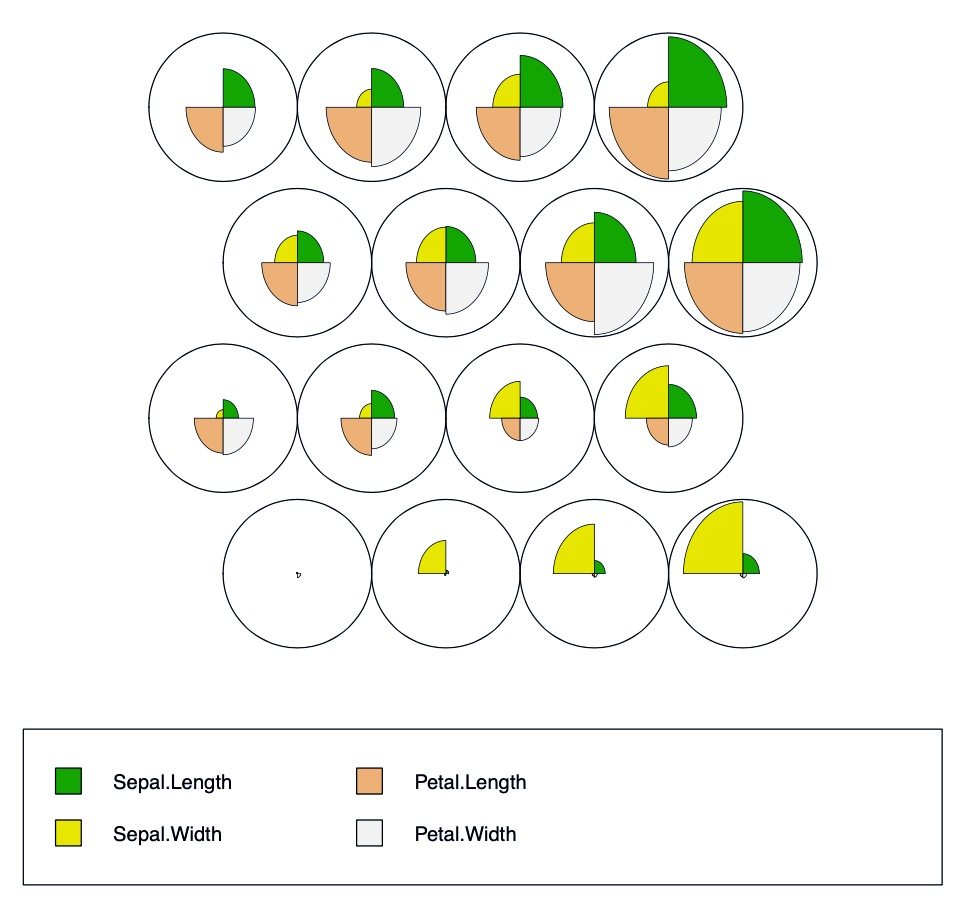
\includegraphics[width=0.6\textwidth]{Som1.jpeg}
\end{center}
\caption[Self Organizing Map Display]{The self organizing map output layer node show the representation of the "winning weight value" inside each circle of the 4x4 hexagonal topology}
\end{figure}

Following the initial training of the SOM, a hierarchical structure is
imposed over the 16 SOM output cluster. The hierarchy here is a
representation of Euclidean distance as measured with respect to the
characteristics of the winning node. A cut value of three clusters is
chosen to represent the three Iris classifications types

\newpage

\begin{figure}[!h]
\begin{center}
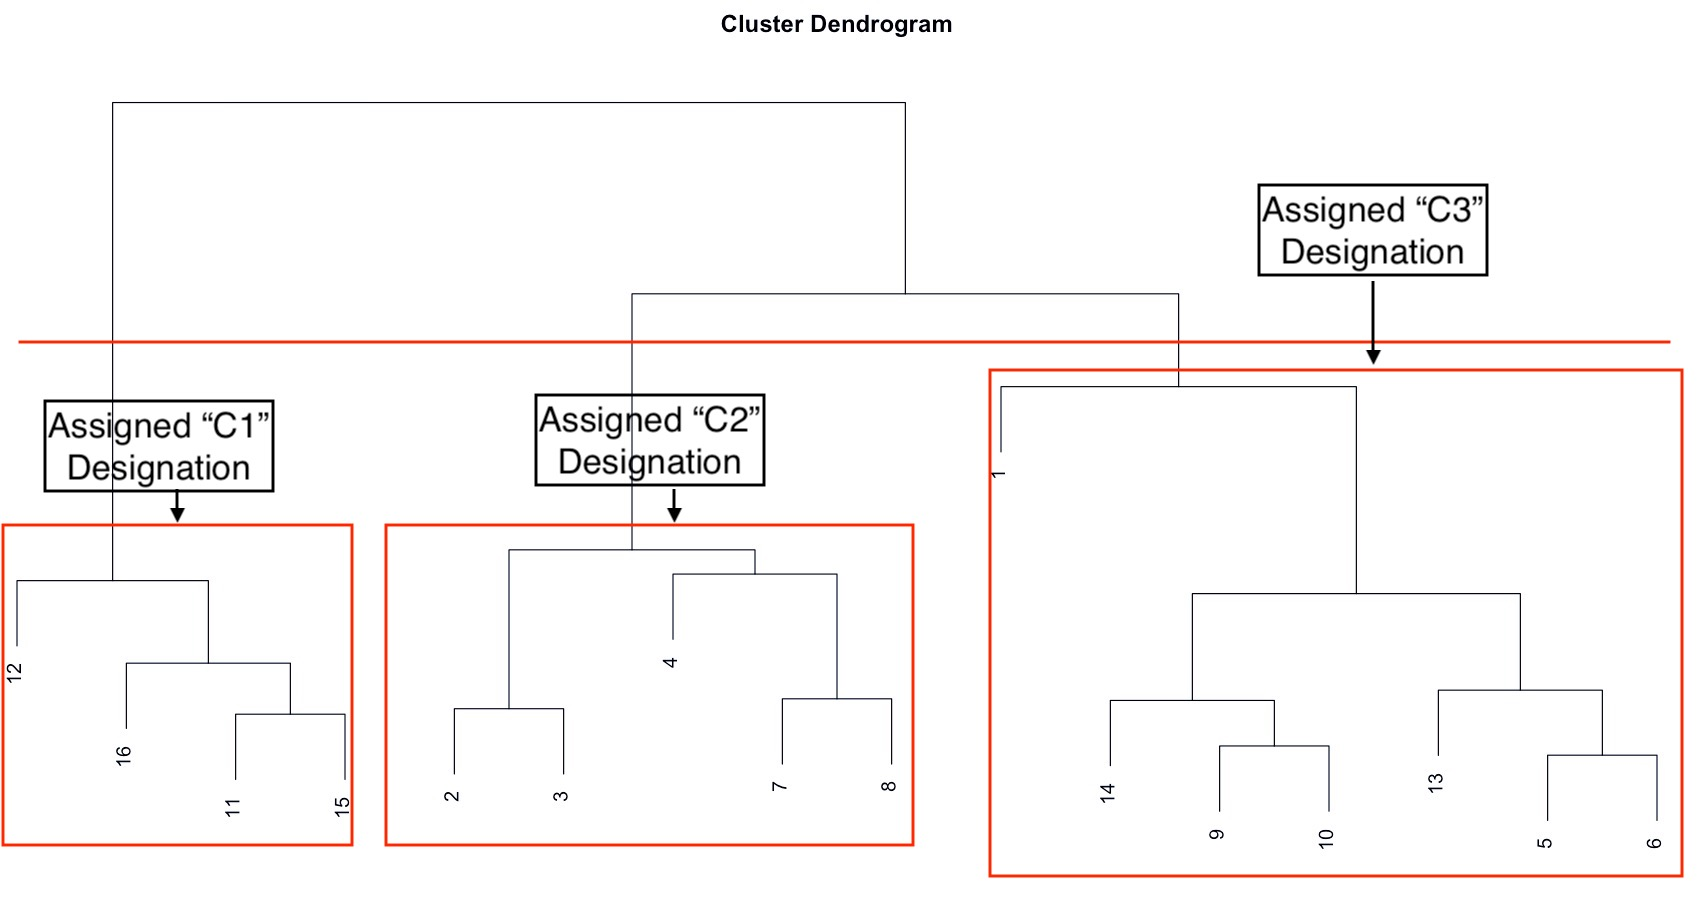
\includegraphics[width=0.75\textwidth]{Dendrogram.jpeg}
\end{center}
\caption[Dendrogram]{The self organizing map output layer nodes are organized into a hierarchy using a Euclidean metric measurement between representative "winning weight values".}
\end{figure}

The goal is now to impose another hierarchy onto this grouping of
clusters.

\begin{table}[h!]
\begin{center}
\begin{tabular}{|c|c|c|}
\hline
Cluster & Mean Sum All & Mean Product  All  \\
\hline
C1 & 3.600  & 1.320  \\
\hline
C2 & 2.680  & 1.010 \\ 
\hline
C2 & 0.039  & 0.030 \\ 
\hline
\end{tabular}
\end{center}
\caption[Meta Variables Grouped by Meta Clusters]{Mean sum of all variable and Mean product of all variables grouped by the clusters in Figure 3}
\end{table}

Figure 4 below indicates that, although not perfectly separable, the
Iris classes are distinguishable based on the fact that there seems to
be a quadratic trend in the value of \textit{Product of All Variables}
when plotted against \textit{Sum of All Variables}. Additionally, this
trend can be approximately partitioned according to Species with

\[
\text{S} \leq \text{Ve} \leq \text{Vi} \tag{EQ 1}
\]

\newpage

\begin{figure}[!h]
\begin{center}
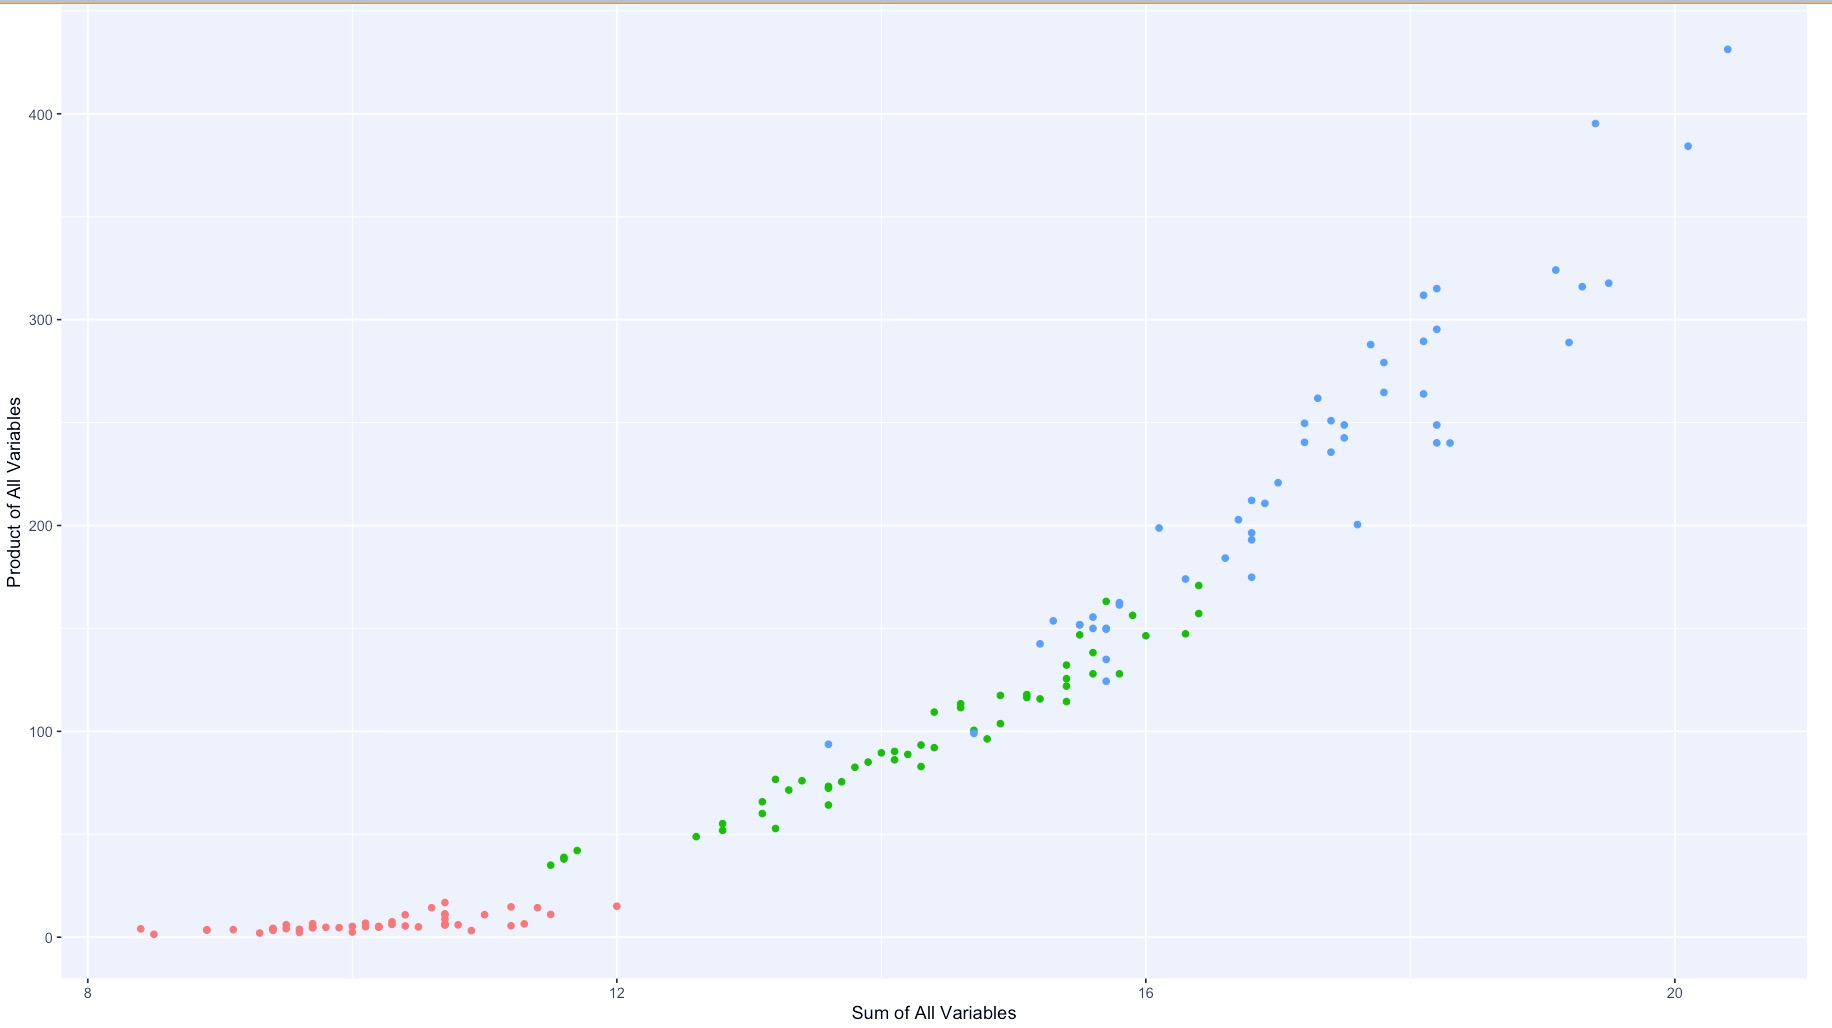
\includegraphics[width=0.75\textwidth]{SumVProd.jpeg}

\vspace{5pt}

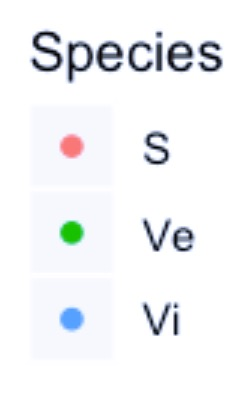
\includegraphics[width=0.1\textwidth]{KeyData.jpeg}
\end{center}
\caption[Iris Data Product Of All Variable Plot]{Plot of all four variables vs Product of All Variables}
\end{figure}

Equation (1) combined with Figure 4 motivates the assignments:

\begin{table}[!h]
\begin{center}
\begin{tabular}{|c|c|}
\hline
Cluster & Assigned Cluster\\
\hline
C1 & Vi  \\
\hline
C2 & Ve  \\ 
\hline
C2 & S  \\ 
\hline
\end{tabular}
\end{center}
\caption[Hierarchical Cluster Assignments]{Assignments from meta variable summaries}
\end{table}

\begin{center}\rule{0.5\linewidth}{\linethickness}\end{center}

\newpage

\hypertarget{discussion}{%
\section{Discussion}\label{discussion}}

This analysis has classified Edgar Anderson's Iris data using a 4x4 Self
Organizing Map. Observations were first separated into test and training
data, with 75\% of the observations being used in the training set. The
16 SOM outcomes were then clustered into three groups using a
hierarchical criteria based on the Euclidean distance from
representative nodes. An Iris species assignment was associated to each
of the three hierarchical clusters by deducing an order present in the
data that was also found in the unlabeled clusters formed from
hierarchical clustering.

After assigning a Species label to the training data values, the cluster
assignments are found to be 77.68\% accurate in classify the correct
training observation, and after evaluating the pre-trained SOM on the
test data in a similar calculation (with only 38 observations to
classify) a 98\% classification accuracy is estimated.

\hypertarget{next-steps}{%
\subsection{Next Steps}\label{next-steps}}

A 98\% test classification accuracy values is not reasonable when
considering 78\% estimated for the training set. This is all in addition
to the fact that minimum classification accuracy should be considered
66\% for any algorithm attempting to classify a three-level set of
observations. Additional consideration needs to be paid to accuracy
estimates conducted over differing training/testing sizes.

\begin{center}\rule{0.5\linewidth}{\linethickness}\end{center}

\newpage

\hypertarget{appendix}{%
\section{Appendix}\label{appendix}}

\hypertarget{appendix-a-data-plots}{%
\subsection{Appendix A: Data Plots}\label{appendix-a-data-plots}}

\textbf{Summary Plots of} \textit{Sum Of All Variables}

\begin{figure}[!h]
\begin{center}
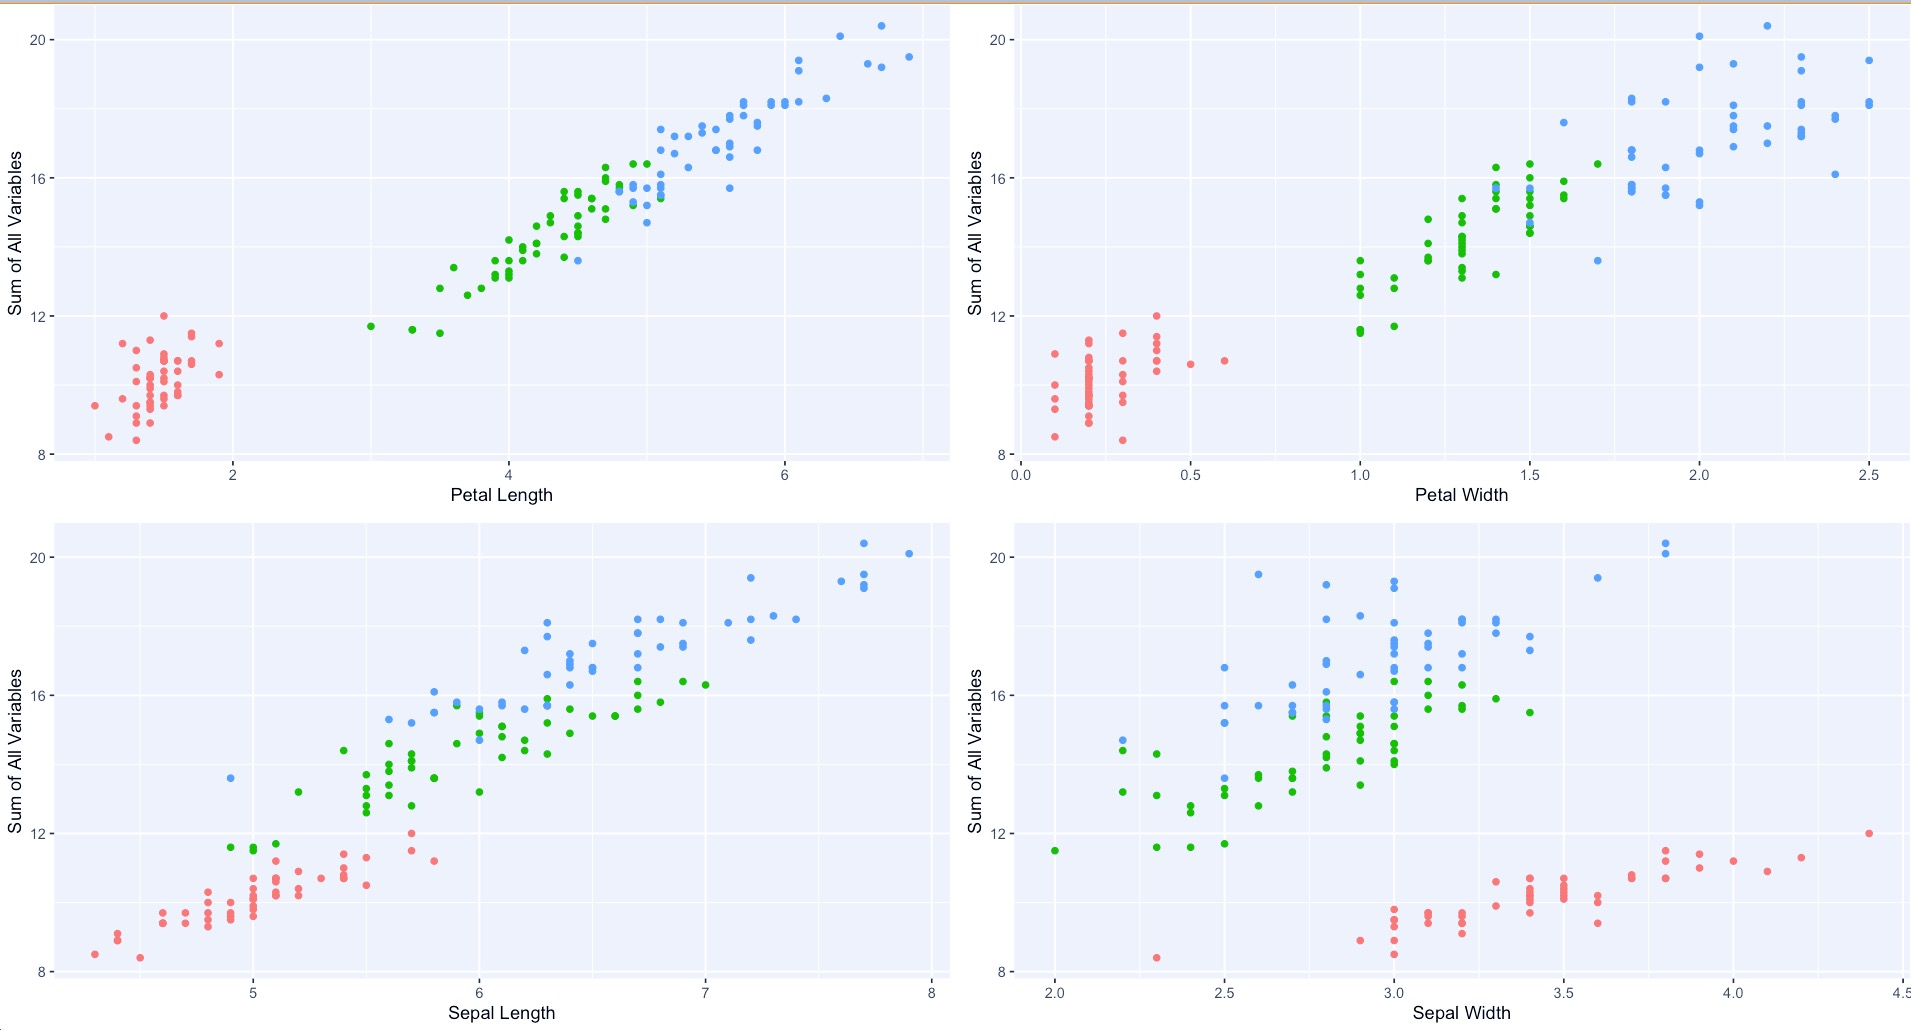
\includegraphics[width=0.75\textwidth]{SumOfAll.jpeg}
\end{center}
\caption[Iris Data Sum Of All Variable Plot]{Plot of all four variables vs Sum of All Variables}
\end{figure}

\textbf{Summary Plots of} \textit{Product Of All Variables}

\begin{figure}[!h]
\begin{center}
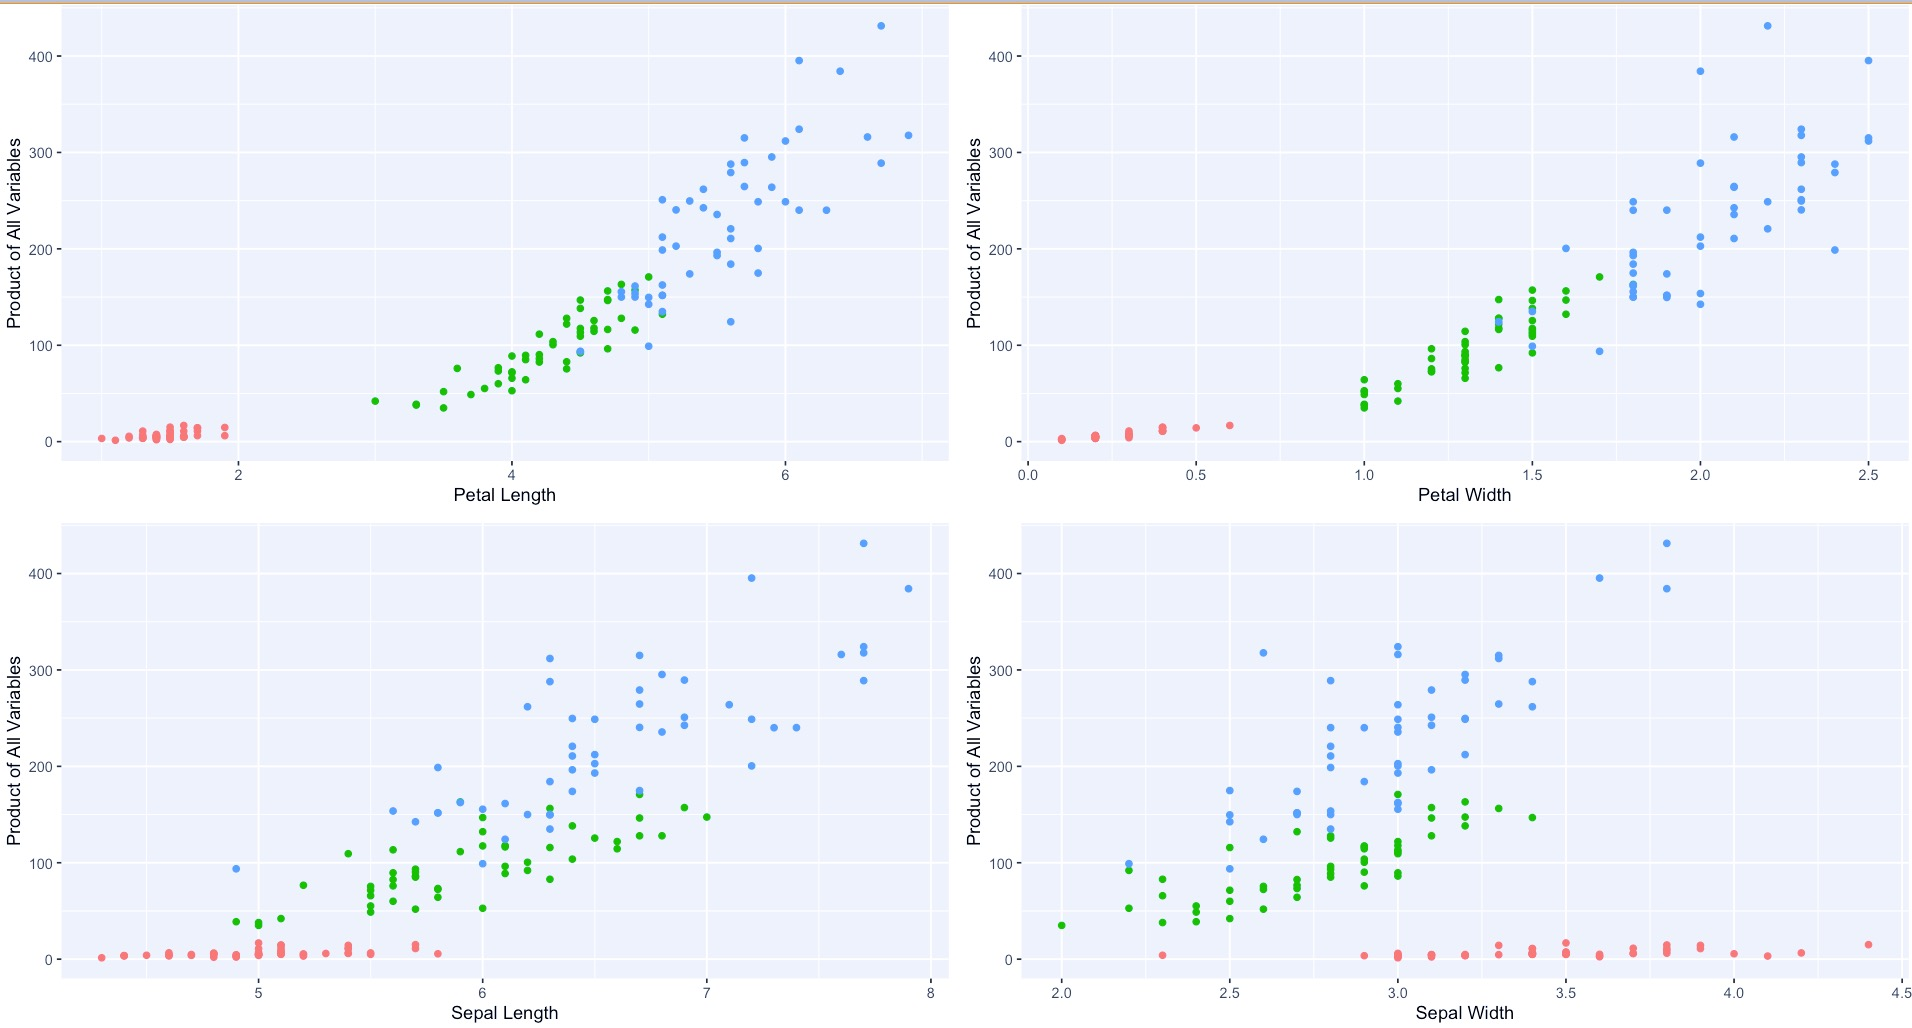
\includegraphics[width=0.75\textwidth]{ProdOfAll.jpeg}
\end{center}
\caption[Iris Data Product Of All Variable Plot]{Plot of all four variables vs Product of All Variables}
\end{figure}

\newpage

\hypertarget{list-of-figures-and-tables}{%
\subsection{List of Figures and
Tables}\label{list-of-figures-and-tables}}

\thispagestyle{empty}

\begin{singlespace}
\listoffigures
\listoftables
\end{singlespace}

\newpage

\hypertarget{data-and-code-availability}{%
\subsection{Data and Code
Availability}\label{data-and-code-availability}}

\thispagestyle{empty}

Access to code, with instructions, and all data used for the analysis
completed here is available for download at:

\texttt{https://github.com/leepanter/SelfOrganizingMaps.git}

or

\texttt{git@github.com:leepanter/SelfOrganizingMaps.git}

\hypertarget{references}{%
\subsection{References}\label{references}}

\bibliography{Bib_AccRefSheet}

\hypertarget{refs}{}
\leavevmode\hypertarget{ref-teuvo1982self}{}%
1. Teuvo K (1982) Self-organized formation of topologically correct
feature maps. \emph{Biological cybernetics} 43: 59--69.

\leavevmode\hypertarget{ref-asan2012introduction}{}%
2. Asan U, Ercan S (2012) An introduction to self-organizing maps, In,
\emph{Computational intelligence systems in industrial engineering},
Springer, 295--315.

\leavevmode\hypertarget{ref-Grey_SelfOrganizing_2020}{}%
3. (2020) \emph{Coloradoedu}.

\leavevmode\hypertarget{ref-larose2014discovering}{}%
4. Larose DT, Larose CD (2014) Discovering knowledge in data: An
introduction to data mining, John Wiley \& Sons.

\leavevmode\hypertarget{ref-Belavkin}{}%
5. Belavkin R Lecture 13: Self-organising maps.


\end{document}
